\begin{definition}{WEB-Architektur}
    \textbf{Client-Server-Modell:}
    \begin{itemize}
        \item Browser (Client) sendet Anfragen an Server
        \item Server verarbeitet Anfragen und sendet Antworten
        \item Kommunikation über HTTP/HTTPS (Port 80/443)
    \end{itemize}
    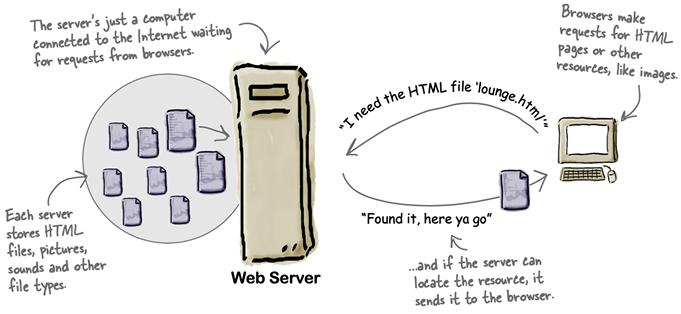
\includegraphics[width=0.8\linewidth]{images/web_architektur.png}
\end{definition}

\begin{concept}{Technologien}

    \textbf{Client-Seitig} $\rightarrow$ Front-end Entwickler
    \begin{itemize}
        \item Beschränkt auf Browser-Funktionalität
        \item Basistechnologien: HTML (Struktur), CSS (Darstellung), JavaScript (Verhalten)
        \item Browser APIs und Web-Standards
    \end{itemize}

    \textbf{Server-Seitig} $\rightarrow$ Back-end Entwickler
    \begin{itemize}
        \item Freie Wahl von Plattform und Programmiersprache
        \item Generiert Browser-kompatible Ausgabe
        \item Beispiele: Node.js, Express, REST APIs
    \end{itemize}
\end{concept}

\begin{concept}{Internet vs. WWW}

    \textbf{Internet:}
    \begin{itemize}
        \item Weltweites Netzwerk aus vielen Rechnernetzwerken
        \item Verschiedene Dienste: E-Mail, FTP, WWW, etc.
        \item Basis-Protokolle: TCP/IP
    \end{itemize}
    
    \textbf{World Wide Web:}
    \begin{itemize}
        \item Service, der auf dem Internet aufbaut
        \item Entwickelt von Tim Berners-Lee am CERN (1990er)
        \item Basiert auf: HTTP, HTML, URLs
    \end{itemize}
\end{concept}

\begin{concept}{Web-Standards}
    \begin{itemize}
        \item W3C (World Wide Web Consortium)
        \item WHATWG (Web Hypertext Application Technology Working Group)
        \item HTML Living Standard
        \item Browser-Hersteller (Chrome, Firefox, Safari, etc.)
    \end{itemize}
\end{concept}